\section{Extraction Process: Other Parts of the Book}
\label{sec:other}

In terms of the complexity needed to represent and extract them, the
remaining parts of the Sbr-Regesten discussed in this chapter are a
lot less involved than the ``Regesten'' and ``Index'' parts.

\subsection{Front Matter}
\label{sec:frontmatter}

The \emph{front matter} section of the Sbr-Regesten contains the full
title of the book, some information about the authors/editors and the
cover art, as well as some acknowledgments about financial support.

\paragraph{XML Schema}

Aside from a \texttt{<frontmatter>} tag for wrapping the front matter
section, the current version of the XML schema does not introduce any
additional markup for representing the front matter of the
Sbr-Regesten.

\paragraph{Extraction}

As contents of the front matter are interspersed with
\href{https://en.wikipedia.org/wiki/Conditional_comment}{conditional
  comments} in the HTML version of the Sbr-Regesten, the extraction
process relies on textual cues that were manually determined to locate
relevant lines in the file. When the
\texttt{frontmatter\_extractor.py} module is loaded, it first reads
the contents of \texttt{html/sbr-regesten.html} and turns it into a
\texttt{BeautifulSoup} instance. It then collects all relevant lines
in a list. As a last step, the \texttt{extract\_frontmatter()}
function takes care of inserting the start tag of the root element
(\texttt{<sbr-regesten>}) into the XML output file and appends the
contents of the front matter.

\subsection{Table of Contents (TOC)}
\label{sec:toc}

The \emph{Table of Contents} lists individual chapters of the
Sbr-Regesten.

\paragraph{XML Schema}

Aside from a \texttt{<toc>} tag for wrapping the Table of Contents,
the current version of the XML schema does not introduce any
additional markup to represent individual entries.

\paragraph{Extraction}

In the HTML source, the \emph{Inhaltsverzeichnis} key word indicates
the start of the table of contents, while the title of the next
chapter (\emph{Vorwort}) indicates the end of the TOC section. These
cues are used by the \texttt{toc\_extractor.py} module to determine
which lines in the HTML source are relevant for the table of contents.
Aside from using different cues, the code for extracting the table of
contents operates in exactly the same way as the extractor responsible
for the front matter section: It reads the HTML source and turns it
into a \texttt{BeautifulSoup} instance, collects all relevant lines
from the textual content of the HTML in a list, and then writes these
lines to the XML output file, wrapping it in the \texttt{<toc>} tag.

\subsection{Preface}
\label{sec:preface}

\emph{Author: Conrad Steffens} \\

\subsection{Bibliography}
\label{sec:bibl}

The \emph{bibliography} section of the Sbr-Regesten lists all
references that are quoted multiple times throughout the text. Entries
in the bibliography section look like this:

\begin{figure}[h]
  \centering
  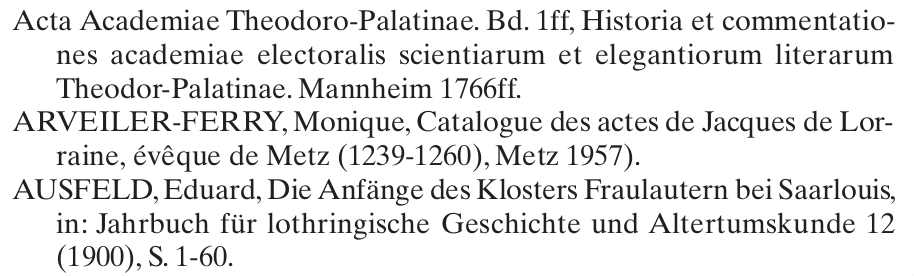
\includegraphics[scale=0.3]{img/bibl-entries}
  \caption{Example entries from the bibliography section of the Sbr-Regesten}
  \label{fig:bibl-entries}
\end{figure}

\paragraph{XML Schema}

The parts of the XML schema for representing the bibliography section
of the Sbr-Regesten are a bit more involved than those for
representing the front matter and TOC sections. As a whole, the
section is wrapped using the \texttt{<listBibl>} tag as suggested by
the TEI guidelines. The title of the bibliography section
(\emph{Literaturverzeichnis}) is taken over from the original text as
is; the XML schema does not define a separate element for it. After
the title, the bibliography section contains a small amount of free
text. In the XML output, this text is wrapped with a tag called
\texttt{<listBibl-info>}. Lastly, individual entries of the
bibliography are annotated using the \texttt{<bibl>} tag whose name
was borrowed from the TEI guidelines and which defines a single
attribute called \texttt{biblidtype} for storing a unique ID for each
entry in the bibliography.

\paragraph{Extraction}

The bibliography is extracted by the module
\texttt{bibliography\_extractor.py}. The module reads the entire HTML
source and turns it into a \texttt{BeautifulSoup} instance. It then
proceeds to split the document up into paragraphs exploiting the
\texttt{<p>} tag in the HTML. Then, the
\texttt{bibliography\_extractor.py} creates a \texttt{<listBibl>} tag.
In order to find the paragraphs relevant to the bibliography it
searches for the keyword \emph{Literaturverzeichnis}. Once this is
found, it starts extracting the bibliography. The first paragraph
following the keyword \emph{Literaturverzeichnis} is tagged as
\texttt{<listBibl-info>} and appended to it. Each of the following
non-empty paragraphs obtains a \texttt{<bibl>} tag with a continuous
id as attribute and is again appended to the \texttt{<listBibl>} tag.
The \texttt{bibliography\_extractor.py} stops when finding the keyword
\emph{Abk}, which is the beginning of the next section of the book.
The created \texttt{BeautifulSoup} instance is
\href{http://www.crummy.com/software/BeautifulSoup/bs4/doc/#pretty-printing}{prettified}
and written into a temporary file. The latter is post-processed for
the purpose of indentation, before the bibliography is finally added
to the \texttt{sbr-regesten.xml}.

\subsection{Abbreviations}
\label{sec:abbrevs}

The \emph{abbreviations} section of the Sbr-Regesten lists
abbreviations used throughout the book, along with their expansions:

\begin{figure}[h]
  \centering
  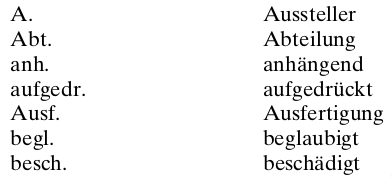
\includegraphics[scale=0.4]{img/abbrevs}
  \caption{Excerpt from the abbreviations section of the Sbr-Regesten}
  \label{fig:abbrevs}
\end{figure}

The XML schema described below for representing this part of the
original text is heavily based on recommendations from the TEI
guidelines.

\paragraph{XML Schema}

For wrapping the abbreviations section as a whole, the XML schema
defines the \texttt{<abbrev-list>} tag. The title of the abbreviations
section (\emph{Abkürzungen}) is inserted into the
\texttt{<abbrev-list>} node as is; the schema does not define a
separate tag for it. By contrast, the free text following the title is
wrapped using the \texttt{<list-info>} tag.\footnote{The name of this
  tag has been kept generic on purpose; it is reused in the list of
  initials described shortly.} Individual entries of the abbreviations
section are represented by \texttt{<entry>} nodes. These nodes have
two child elements each, one for tagging the abbreviation itself,
called \texttt{abbr}, and one for tagging its expansion, called
\texttt{expan}.

\paragraph{Extraction}

The \texttt{abbrev\_extractor.py} module uses the titles of the
abbreviations section and the section which succeeds it
(\emph{Abkürzungen} and \emph{Siglen}, respectively) to identify
relevant lines in the HTML source; any textual content between these
two keywords is considered to belong to the abbreviations section. The
extraction algorithm is similar to the algorithms used for extracting
front matter and TOC sections: First, using the cues described above
and ignoring empty lines, a list of relevant lines is accumulated from
a \texttt{BeautifulSoup} instance representing the HTML source. Then,
abbreviations and their expansions are annotated with the
corresponding tags and written to the XML output file one by one.

\subsection{Initials}
\label{sec:initials}

The \emph{initials} section of the Sbr-Regesten lists author initials
that are used throughout the book, along with their expansions:

\begin{figure}[h]
  \centering
  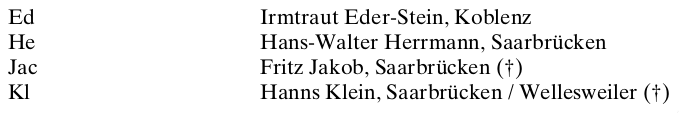
\includegraphics[scale=0.4]{img/initials}
  \caption{Initials section of the Sbr-Regesten}
  \label{fig:initials}
\end{figure}

\paragraph{XML Schema}

For wrapping the initials section as a whole, the XML schema defines
an element called \texttt{initials-list}. The \emph{type} of this
element is the same as the one used for the abbreviations section. As
a result, the inner structure of the \texttt{<initials-list>} node in
the XML output is identical to that of the \texttt{<abbrev-list>} node
discussed in section \ref{sec:abbrevs}, and does not need to be
discussed again here.

\paragraph{Extraction}

The \texttt{} module uses the title of the initials section
(\emph{Siglen}) and the title of the first regest to detect content
belonging to the initials section in the HTML source. Aside from some
adjustments that had to be made due to the fact that the initials
section lacks an info section, the algorithm for extracting and
annotating initials and their expansions is virtually identical to the
one used for the abbreviations section.

\subsection{Archives}
\label{sec:archives}

\emph{Author: Conrad Steffens} \\

\subsection{Future Work: DRYing Out Extractor Modules}
\label{sec:future-work-other}

Due to time constraints it was not possible to refactor the modules
responsible for extracting the parts of the Sbr-Regesten discussed in
this chapter. As a result, there is a fair amount of code duplication
within and between individual extractor modules. Since they contain
fairly small amounts of code, this is not a critical issue, but if the
extraction process is to be extended in the future, it would be
desirable to
\href{https://en.wikipedia.org/wiki/Don't_repeat_yourself}{DRY} out
the existing code beforehand.
